\subsubsection{Caso d'uso UC8.2.1.2: Modifica domanda a risposta multipla}
	\label{UC8.2.1.2}
	\begin{figure}[h]
		\centering
			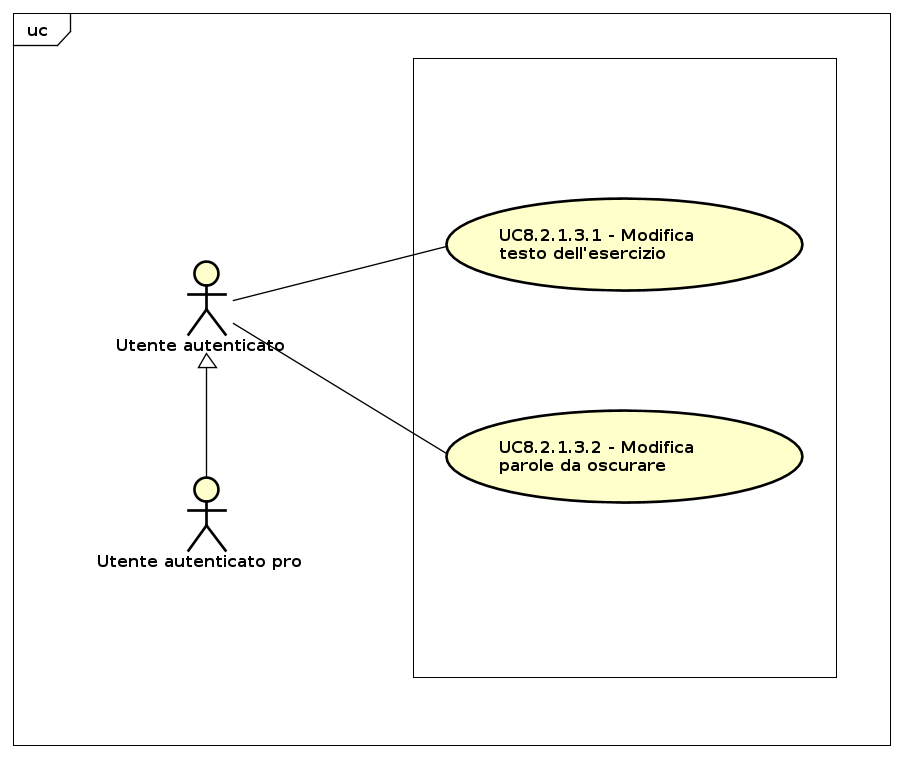
\includegraphics[scale=0.45,keepaspectratio]{UML/UC8_2_1_2.png}
		\caption{UC8.2.1.2: Modifica domanda a risposta multipla}
	\end{figure}
	\FloatBarrier
	\begin{itemize}
		\item
			\textbf{Attori}: utente autenticato, utente autenticato pro;
		\item		
			\textbf{Descrizione}: lo scopo di questa funzionalità è offrire agli attori la possibilità di modificare una domanda a risposta multipla;
		\item
			\textbf{Precondizione}: gli attori hanno selezionato la seguente funzionalità; 
		\item
			\textbf{Postcondizione}: gli attori hanno modificato una domanda a risposta multipla;
		\item
			\textbf{Scenario principale}:
	       		\begin{enumerate}
	       			\item
	       			Gli attori possono modificare il testo della domanda (UC8.2.1.2.1)
	       			\item
	       			Gli attori possono modificare l'immagine (UC8.2.1.2.2)
	       			\item
	       			Gli attori possono modificare le opzioni di risposta (UC8.2.1.2.3);
					\item
					Gli attori possono modificare le risposte corrette (UC8.2.1.2.4).
	 			\end{enumerate}
	\end{itemize}

\subsubsection{Caso d'uso UC8.2.1.2.1: Modifica testo della domanda}
	\begin{itemize}
		\item
			\textbf{Attori}: utente autenticato, utente autenticato pro;
		\item		
			\textbf{Descrizione}: lo scopo di questa funzionalità è offrire agli attori la possibilità di modificare il testo della domanda;
		\item
			\textbf{Precondizione}: gli attori hanno selezionato la modalità di modificare una domanda a risposta multipla; 
		\item
			\textbf{Postcondizione}: gli attori hanno modificato il testo della domanda;
		\item
			\textbf{Scenario principale}: gli attori modificano il testo della domanda. 
	 			
	\end{itemize}
	
\subsubsection{Caso d'uso UC8.2.1.2.2: Modifica immagine}
	\begin{itemize}
		\item
			\textbf{Attori}: utente autenticato, utente autenticato pro;
		\item		
			\textbf{Descrizione}: lo scopo di questa funzionalità è offrire agli attori la possibilità di modificare l'immagine relativa al testo della domanda;
		\item
			\textbf{Precondizione}: gli attori hanno selezionato la funzionalità di modificare una domanda a risposta multipla; 
		\item
			\textbf{Postcondizione}: gli attori hanno modificato l'immagine;
		\item
			\textbf{Scenario principale}: gli attori modificano l'immagine. 	
	\end{itemize}
	
	
\subsubsection{Caso d'uso UC8.2.1.2.3: Modifica opzioni di risposta}
	\begin{itemize}
		\item
			\textbf{Attori}: utente autenticato, utente autenticato pro;
		\item		
			\textbf{Descrizione}: lo scopo di questa funzionalità è offrire agli attori la possibilità di modificare le opzioni di risposta;
		\item
			\textbf{Precondizione}: gli attori hanno selezionato la funzionalità di modificare una domanda a risposta multipla; 
		\item
			\textbf{Postcondizione}: gli attori hanno modificato le opzioni di risposta;
		\item
			\textbf{Scenario principale}:
	       		\begin{enumerate}
	       			\item
	       			Gli attori possono modificare opzioni di risposta che includono testo (UC8.2.1.2.3.1);
					\item
					Gli attori possono modificare opzioni di risposta che includono immagini (UC8.2.1.2.3.2).
	 			\end{enumerate}
	\end{itemize}	
	
\subsubsection{Caso d'uso UC8.2.1.2.3.1: Modifica opzioni di risposta che includono testo}
	\begin{itemize}
		\item
			\textbf{Attori}: utente autenticato, utente autenticato pro;
		\item		
			\textbf{Descrizione}: lo scopo di questa funzionalità è offrire agli attori la possibilità di modificare le opzioni di risposta che includono testo;
		\item
			\textbf{Precondizione}: gli attori hanno selezionato la funzionalità di modificare una domanda a risposta multipla con opzioni di risposta che includono testo; 
		\item
			\textbf{Postcondizione}: gli attori hanno modificato le opzioni di risposta che includono testo;
		\item
			\textbf{Scenario principale}: gli attori modificano le opzioni di risposta che includono testo. 			
	\end{itemize}	
	
\subsubsection{Caso d'uso UC8.2.1.2.3.2: Modifica opzioni di risposta che includono immagini}
	\begin{itemize}
		\item
			\textbf{Attori}: utente autenticato, utente autenticato pro;
		\item		
			\textbf{Descrizione}: lo scopo di questa funzionalità è offrire agli attori la possibilità di modificare le opzioni di risposta che includono immagini;
		\item
			\textbf{Precondizione}: gli attori hanno selezionato la funzionalità di modificare una domanda a risposta multipla con opzioni di risposta che includono immagini; 
		\item
			\textbf{Postcondizione}: gli attori hanno modificato le opzioni di risposta che includono immagini;
		\item
			\textbf{Scenario principale}: gli attori modificano le opzioni di risposta che includono immagini. 			
	\end{itemize}
	
\subsubsection{Caso d'uso UC8.2.1.2.4: Modifica risposte corrette}
	\begin{itemize}
		\item
			\textbf{Attori}: utente autenticato, utente autenticato pro;
		\item		
			\textbf{Descrizione}: lo scopo di questa funzionalità è offrire agli attori la possibilità di modificare la selezione delle risposte corrette;
		\item
			\textbf{Precondizione}: gli attori hanno selezionato la funzionalità di modificare domande a risposte multiple; 
		\item
			\textbf{Postcondizione}: gli attori hanno modificato la selezione delle risposte corrette;
		\item
			\textbf{Scenario principale}: gli attori modificano la selezione delle risposte corrette. 			
	\end{itemize}

	
	
	
	
	
	
	